\documentclass[a4paper,11pt]{article}

% Identificação
\newcommand{\pbtitulo}{CMS e ECM}
\newcommand{\pbversao}{1.0}

\usepackage{../sty/tutorial}

%----------------------------------------------------------------------
% Início do Documento
%----------------------------------------------------------------------
\begin{document}
	
\maketitle % mostrar o título
\thispagestyle{fancy} % habilitar o cabeçalho/rodapé das páginas

%----------------------------------------------------------------------
% RESUMO DO ARTIGO
%----------------------------------------------------------------------

\begin{abstract}	
	\initial{N}a vida real existem diversos cenários para uma empresa, um desses passa por um CMS e outro por um ECM. Ainda sem ideia do que me refiro? Pense em um CMS como um portal de conteúdo, enquanto que um ECM está mais para um grande conjunto de documentos, mas não apenas documentos, tudo o que envolve ao seu redor como guardá-lo e manter suas diversas versões de modificação, facilidades de pesquisa e eliminação. Esta apostila busca um meio de juntar os dois dos mais populares CMS e ECM livres, rápidos e em Java. Liferay DXP e Alfresco.
\end{abstract}

%----------------------------------------------------------------------
% CONTEÚDO DO ARTIGO
%----------------------------------------------------------------------
\section{CMS - Liferay DXP}
\textbf{Liferay DXP} (\textit{Digital Experience Platform}) é uma poderosa solução de gestão de conteúdo (CMS) projetada para a criação de experiências digitais personalizadas e integradas. Como um \textbf{CMS} (\textit{Content Management System}), destaca-se por sua capacidade de gerenciar grandes volumes de conteúdo com eficiência, oferece ferramentas que facilitam a criação, organização e publicação de materiais em diversos canais. Além disso, permite que as empresas construam portais, intranets, sites corporativos e aplicações Web ricas, garante assim flexibilidade e adaptabilidade às necessidades específicas de cada negócio.
\begin{figure}[!htb]
	\centering
	
\includegraphics[width=0.4\textwidth]{imagens/LogoLiferay}
	\caption{Logo do Liferay}
\end{figure}

Uma das principais vantagens do \textbf{Liferay} é sua arquitetura modular e altamente personalizável. Suporta integrações com uma ampla gama de sistemas legados, APIs e serviços externos, promove uma centralização de informações e processos. Outra característica é sua escalabilidade, que atende desde pequenas empresas até corporações globais. Além disso, oferece ferramentas de análise integradas, e auxilia as organizações a entender melhor o comportamento dos usuários e a melhorar continuamente a experiência digital oferecida.

Outro grande diferencial do \textbf{Liferay} é sua robusta funcionalidade para personalização e segmentação de conteúdo. Utiliza dados do usuário para entregar experiências únicas e adaptadas a diferentes perfis, o que é essencial em estratégias de marketing digital modernas. O sistema também é reconhecido por sua segurança avançada e conformidade com regulamentações como o GDPR (\textit{General Data Protection Regulation}), garantindo a proteção dos dados. Com suporte a uma comunidade global de desenvolvedores e uma sólida base de documentação, o \textbf{Liferay} oferece um ecossistema confiável para empresas que buscam otimizar sua presença digital.

\section{ECM - Alfresco}
\textbf{Alfresco} é uma renomada plataforma de \textbf{ECM} (\textit{Enterprise Content Management}), projetada para auxiliar as organizações a gerenciar documentos e processos empresariais de forma eficiente. Se destaca por oferecer uma solução robusta para armazenar, organizar e recuperar conteúdos corporativos, incluindo documentos, imagens e registros. Sua interface intuitiva e funcionalidades avançadas permite que as empresas centralizem o controle de suas informações, reduzam a redundância de dados e aumentem a produtividade.
\begin{figure}[!htb]
	\centering
	
\includegraphics[width=0.5\textwidth]{imagens/LogoAlfresco}
	\caption{Logo do Alfresco}
\end{figure}

Uma de suas grandes vantagens é a capacidade de automatizar processos empresariais por meio de fluxos de trabalho inteligentes. Integra ferramentas como \textbf{OCR} (reconhecimento óptico de caracteres) e suporte a metadados, facilita a classificação e pesquisa de documentos. Além disso, sua compatibilidade com padrões abertos, como \textbf{CMIS}\footnote{CMIS é um padrão \textbf{OASIS} de software livre que permite que aplicativos trabalhem com um ou mais sistemas de gerenciamento de conteúdo. CMIS define um modelo de domínio padrão e um conjunto de serviços e ligações de protocolo para Web e RESTful AtomPub.} (\textit{Content Management Interoperability Services}), e integração com sistemas legados tornam o \textbf{Alfresco} uma escolha flexível para empresas que precisam unificar suas operações em um único ambiente digital. A escalabilidade da plataforma permite atender desde pequenas empresas até grandes corporações, com capacidade para armazenar milhões de documentos.

Outro ponto de destaque do \textbf{Alfresco} é sua abordagem à segurança e conformidade regulatória. A plataforma oferece recursos avançados para controle de acesso, auditoria e gerenciamento de permissões, garante que dados sensíveis sejam protegidos contra acessos não autorizados. Além disso, suporta a conformidade com regulamentações como \textbf{GDPR} (\textit{General Data Protection Regulation}) e \textbf{HIPAA} (\textit{Health Insurance Portability and Accountability Act}), o que o torna ideal para setores como saúde, financeiro e jurídico. Com uma forte comunidade de desenvolvedores e parceiros, o \textbf{Alfresco} oferece suporte contínuo e inovação constante, sendo uma solução confiável para empresas que buscam eficiência e governança no gerenciamento de seus conteúdos empresariais.

\textbf{ATENÇÃO}: Antes mesmo de começarmos qualquer processo de instalação ou configuração saiba que essas são ferramentas que consomem recursos, principalmente de memória, então é recomendável que a máquina possua ao menos 16 Gb de memória, ou que a instalação seja realizada em 2 máquinas com 4 Gb que se comunicam via rede, onde uma delas conterá o \textbf{Liferay} e outra o \textbf{Alfresco}.

\section{E na prática?}
Tudo isso é muito fantástico mas porquê trabalhar separadamente um \textbf{CMS} e \textbf{ECM}? integrar o \textbf{Liferay DXP} e o \textbf{Alfresco} pode ser uma estratégia altamente vantajosa para empresas que buscam otimizar a gestão de conteúdos e oferecer experiências digitais mais ricas e personalizadas. Enquanto o \textbf{Liferay DXP} se destaca como uma plataforma voltada para a criação de portais, sites e intranets, \textbf{Alfresco} é uma solução especializada no armazenamento, organização e controle de documentos. Essa integração combina o melhor dos dois mundos: a capacidade de gerenciar grandes volumes de documentos e processos empresariais do Alfresco com a interface amigável e personalizável do Liferay, que facilita o acesso e a entrega de conteúdo ao usuário final.
\begin{figure}[!htb]
	\centering
	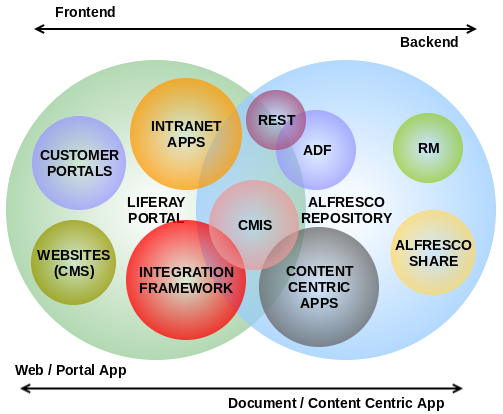
\includegraphics[width=0.7\textwidth]{imagens/AlfeLif}
	\caption{Liferay e Alfresco juntos}
\end{figure}

Uma das principais razões para integrar essas ferramentas é a centralização e unificação do conteúdo. \textbf{Alfresco} pode servir como o repositório central de documentos, registros e outros ativos corporativos, enquanto \textbf{Liferay} utiliza esses dados para enriquecer a experiência do usuário nos diversos canais digitais. Por exemplo, documentos armazenados, como relatórios, contratos ou manuais, podem ser apresentados de forma dinâmica em portais, com controles de acesso e personalização baseados no perfil do usuário. Isso não apenas melhora a eficiência operacional, como garante a consistência e a segurança no acesso das informações.

Além disso, a integração promove maior automação e colaboração nos fluxos de trabalho empresariais. Processos gerenciados no Alfresco, como aprovações de documentos ou arquivamento automático, podem ser acionados diretamente por meio do Liferay, isso proporciona uma experiência mais fluida para os usuários. Essa sinergia permite que as empresas aproveitem ao máximo as funcionalidades de cada plataforma, otimizando a produtividade, reduzindo custos operacionais e entregando mais valor ao cliente final. Com essa combinação, as organizações conseguem alinhar a gestão de conteúdos corporativos à criação de experiências digitais modernas e engajadoras.

\section{E isso tudo em contêineres do Docker}
Docker, como plataforma de contêineres, oferece uma maneira rápida e flexível de empacotar, distribuir e executar aplicações em ambientes isolados. Ao utilizar Docker para orquestrar a integração entre Liferay DXP e Alfresco, as empresas podem garantir uma configuração mais ágil, consistência nos ambientes de desenvolvimento, testes e produção, além de facilitar o escalonamento das aplicações conforme necessário.

Uma das principais vantagens de usar Docker nessa integração é a simplificação do processo de deployment. Com o Docker, tanto o Liferay DXP quanto o Alfresco podem ser configurados e executados em contêineres isolados, o que facilita o gerenciamento de dependências e versões. Isso elimina conflitos de ambiente que poderiam ocorrer ao rodar as aplicações em servidores tradicionais. Além disso, a utilização de contêineres permite que cada ferramenta seja executada com a sua própria configuração e requisitos de infraestrutura, enquanto ainda mantém a comunicação entre elas de forma eficaz e segura. Isso reduz o risco de erros e aumenta a previsibilidade no desenvolvimento.

Outro benefício é a flexibilidade de escalabilidade. Quando uma das ferramentas, como o Alfresco, precisar de mais recursos de processamento ou armazenamento, a solução pode ser escalada facilmente sem impactar o funcionamento do Liferay DXP, graças à natureza isolada dos contêineres. Docker também facilita o gerenciamento de clusters e a replicação de ambientes em diferentes servidores ou nuvens, permite uma melhor utilização dos recursos e garante a tão sonhada "alta disponibilidade".

\subsection{Instalar o Liferay no Docker}
Instalar o Liferay a partir do Docker e um dos trabalhos mais fáceis que podem ser realizados por um desenvolvedor, talvez trocar a lâmpada seja mais fácil. Com o simples comando: \\
\codigo{\$ docker run -it -d -m 4g -p 8081:8080 --name=meu-liferay -e JAVA\_VERSION=zulu21 -v /home/[usuario]/liferaymnt:/mnt/liferay liferay/portal:latest}

Basicamente, definimos um contêiner que utiliza 4 gigabytes de memória, que será executado na porta \textbf{8081} (pois a porta 8080 será do Alfresco), que executará o Java 21 e se chamará meu-liferay.

Para interromper o contêiner: \\
\codigo{\$ docker stop meu-liferay}

Para reiniciar o contêiner: \\
\codigo{\$ docker start meu-liferay}

Testemos para ver se funciona corretamente, no navegador acessar o endereço: \url{http://localhost:8081}, o usuário padrão é \textbf{test@liferay.com}, e a senha: \textbf{test}.

\textbf{ATENÇÃO}: Na primeira vez que se logar será forçado para mudar a senha, troque-a para \textbf{admin} (toda em minúsculas), uma vez que entrou corretamente com a nova senha, no perfil em \textit{User Profile} devemos modificar o Screen Name de \textbf{test} para \textbf{admin} (também toda em minúsculas), salvar e confirmar a mudança com a senha.

\subsection{Instalar o Alfresco no Docker}
Subir um Alfresco não é tão simples como o Liferay pois são diversos componentes incluindo o Banco Postgres, Apache Solr e o servidor de mensagens ActiveMQ. Assim o melhor modo e colocá-lo sobre o Docker Compose de modo a gerenciar toda essa informação e trabalhar de modo unido.

Faça um clone do repositório oficial da comunidade no Git: \\
\codigo{\$ git clone https://github.com/Alfresco/acs-deployment.git}

Entre no diretório do Docker Compose: \\
\codigo{\$ cd acs-deployment/docker-compose}

Crie e suba os contêineres necessários: \\
\codigo{\$ docker compose -f community-docker-compose.yaml up}

Para interromper os contêineres: \\
\codigo{\$ docker compose -f community-docker-compose.yaml stop}

Para reiniciá-los: \\
\codigo{\$ docker compose -f community-docker-compose.yaml start}

Testemos para ver se funciona corretamente, no navegador acessar o endereço: \url{http://localhost:8080/alfresco}, o usuário padrão é \textbf{admin}, e a senha: \textbf{admin}.

Outros endereços úteis são: \vspace{-1em}
\begin{itemize}
	\item Control Center \url{http://localhost:8080/admin}
	\item Share \url{http://localhost:8080/share}
	\item Alfresco Content App \url{http://localhost:8080/content-app}
	\item Search Services administration \url{http://localhost:8083/solr}
\end{itemize}

Lembre-se sempre de estar, obrigatoriamente, neste diretório para realizar essas operações.

Outro passo extremamente importante é colocar o Liferay na mesma rede que o Alfresco. Primeiro vamos verificar as redes: \\
\codigo{\$ docker network ls}

Provavelmente deve existir uma rede chamada docker-compose\_default, vamos associar o contêiner do Liferay a esta: \\
\codigo{\$ docker network docker-compose\_default meu-liferay}

\section{Configurar a autenticação do Liferay}
O primeiro passo que devemos proceder para que tudo funcione corretamente é que o usuário administrador do \textbf{Liferay} deve ser o mesmo do \textbf{Alfresco}, pois dessa forma não realizamos autenticações separadamente, por isso ao término da instalação do \textbf{Liferay} garantimos que o usuário e sua senha são \textbf{admin} (que corresponde ao padrão contidos no \textbf{Alfresco}). Agora devemos mudar a forma como o usuário do \textbf{Liferay} se autentica que é por \textbf{e-mail}, enquanto que o \textbf{Alfresco} realiza esse processo por \textbf{nome de usuário}.

Aqui temos um "pulo do gato", o contêiner tanto do \textbf{Liferay} quanto do \textbf{Alfresco} não possuem nenhum editor instalado, ou mesmo, a possibilidade em se instalar um, então os arquivos devem ser criados na máquina local e em seguida copiados para o contêiner nos locais indicados.

Devemos criar um arquivo local com o seguinte conteúdo:
\begin{lstlisting}
layout.show.portlet.access.denied=true
session.store.password=true
company.security.auth.type=screenName
web.server.host=<IP-DA-MAQUINA>
\end{lstlisting}

Na propriedade \textbf{web.server.host} devemos colocar o endereço IP da máquina onde o contêiner do \textbf{Liferay} está executando.

Este arquivo deve ser salvo com o nome \textbf{portal-ext.properties}. Próximo passo é copiá-lo para o contêiner do Liferay: \\
\codigo{\$ docker cp portal-ext.properties meu-liferay:/opt/liferay/tomcat/webapps/ROOT\\/WEB-INF/classes}

Este comando deve retornar a mensagem: \\
\codigo{Successfully copied 2.05kB to meu-liferay:/opt/liferay/tomcat/webapps/ROOT\\/WEB-INF/classes}

Por fim, devemos reiniciar o contêiner do Liferay: \\
\codigo{\$ docker restart meu-liferay}

E uma vez ativo, devemos conseguir logar com o \textit{UserName} \textbf{admin} e mesma senha. E se tudo está funcionando corretamente o Liferay deve ser acessível tanto pelo endereço \url{http://localhost:8081} quanto por \url{http://[IP-MAQUINA]:8081}, isso é importante quando desejamos usar duas máquinas na mesma rede.

\section{Preparar o Alfresco}
A comunicação pode ser realizada de duas formas, a primeira é por \textbf{Web Scripts} isso significa escrevê-los e disponibilizá-los como funcionalidades, por exemplo, desejamos ter uma simples listagem dos documentos disponíveis, ou uma pesquisa personalizada, veremos essa forma em breve. A segunda é por meio de um repositório de interligação através da comunicação \textbf{CMIS}.
\begin{figure}[!htb]
	\centering
	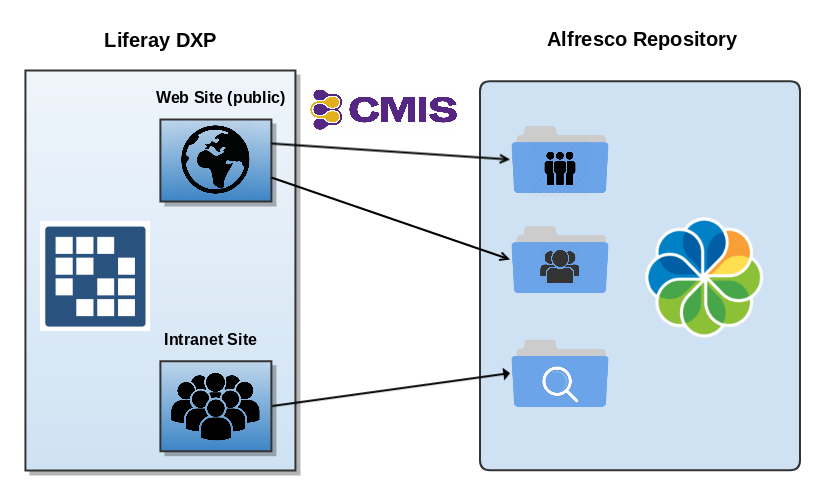
\includegraphics[width=0.6\textwidth]{imagens/IntegraAlfLife}
	\caption{Integração Liferay e Alfresco via CMIS}
\end{figure}

Podemos dizer que esse é um modelo de integração total, onde o usuário do \textbf{Liferay} teria permissão de realizar qualquer processo dentro do \textbf{Alfresco}.

Devemos criar um arquivo com o seguinte conteúdo:
\begin{lstlisting}
cmis.enabled=true
\end{lstlisting}

Este arquivo deve ser salvo com o nome \textbf{alfresco-global.properties}. Próximo passo é copiá-lo para o contêiner do \textbf{Alfresco}: \\
\codigo{\$ docker cp alfresco-global docker-compose-alfresco-1:/usr/local/tomcat/shared\\/classes}

\section{Conclusão}
Em diferentes cenários, \textit{Digital Experience Platforms} como o \textbf{Liferay DXP} (algum tempo atrás conhecido como \textit{Enterprise Portals}), e um \textit{Content Services Platforms} como o \textbf{Alfresco} convivendo juntos e gerenciando partes do ciclo da vida de documentos. A integração via portlet providencia uma solução para o publicador de conteúdo via \textbf{CMIS API}.

Ao utilizar \textbf{Docker} para integrar \textbf{Liferay} e \textbf{Alfresco}, as organizações podem não apenas melhorar a eficiência operacional, mas também garantir uma arquitetura mais resiliente, fácil de manter e expandir à medida que as necessidades do negócio evoluem. 

Sou um entusiasta do mundo \textbf{Open Source} e novas tecnologias. Qual a diferença entre Livre e Open Source? \underline{Livre} significa que esta apostila é gratuita e pode ser compartilhada a vontade. \underline{Open Source} além de livre todos os arquivos que permitem a geração desta (chamados de arquivos fontes) devem ser disponibilizados para que qualquer pessoa possa modificar ao seu prazer, gerar novas, complementar ou fazer o que quiser. Os fontes da apostila (que foi produzida com o LaTex) está disponibilizado no GitHub \cite{github}. Veja ainda outros artigos que publico sobre tecnologia através do meu Blog Oficial \cite{fernandoanselmo}.

%-----------------------------------------------------------------------------
% REFERÊNCIAS
%-----------------------------------------------------------------------------
\begin{thebibliography}{7}
  \bibitem{liferay} 
  Site oficial do Liferay \\
  \url{https://www.liferay.com/}

  \bibitem{alfresco} 
  Site oficial do Alfresco Community Edition \\
  \url{https://docs.alfresco.com/content-services/community/}
  
  	\bibitem{fernandoanselmo} 
	Fernando Anselmo - Blog Oficial de Tecnologia \\
	\url{http://www.fernandoanselmo.blogspot.com.br/}
	
	\bibitem{publicacao} 
	Encontre essa e outras publicações em \\
	\url{https://cetrex.academia.edu/FernandoAnselmo}
	
	\bibitem{github} 
	Repositório para os fontes da apostila \\
	\url{https://github.com/fernandoans/publicacoes}
\end{thebibliography}

\end{document}
